\chapter{Domain combination and relationships}

We continue our investigation of the fundamental mathematical structures for experimental science by studying what happens when we have more than one experimental domain. We will define \textbf{experimental relationships} between experimental domains, which capture either causal or inference relationships between them. We will see that these correspond to continuous functions in the natural topology.

We will take two or more domains and merge all the experimental information that can be gathered through them into a \textbf{combined domain}. We will study how the set of possibilities of the combined domain depends not only on the original domains, but also on the relationships between them. These will also determine the natural topology that can vary from the product topology all the way to the disjoint union topology.

We will also show that experimental relationships, under suitable conditions, can themselves be verified experimentally by constructing the \textbf{relationship domain} for which its possibilities correspond to the possible relationships.

\section{Dependence and equivalence between domains}

The first thing we want to be able to characterize, when dealing with more than one domain, is when there exists a relationship between them. For example, consider the domains for the temperature and height of a mercury column or the domains for the temperature and density of water. How do we express, in this framework, the fact that these domains are connected?

We have two ways to define these relationships between domains. The first is in terms of inference: any measurement on the height of a mercury column is an indirect measurement on its temperature; any experimental test on the density of water is an indirect experimental test on its temperature. The second is in terms of causes: the height of the mercury column depends on its temperature; the density of water is a function of its temperature. The main result of this section is to show that these definitions are equivalent and that the dependent domain can be seen as a sub-domain of the other.

Suppose $\edomain_X$ represents the domain for the temperature of a mercury column while $\edomain_Y$ represents the domain for its height. Since we know that an increase in temperature makes the metal expand, we can infer the temperature of the mercury column by looking at its height. For example, if we verify that \statement{the height of the mercury column is between 24 and 25 millimeters} we will be able to infer that \statement{the temperature is between 24 and 25 Celsius}. That is, given a verifiable statement $\stmt_Y$ we have another verifiable statement $\stmt_X$ that is going to be true if and only if the first one is, that is $\stmt_Y\equiv\stmt_X$.

Note that the inference is between verifiable statements and not intervals. For example, the verifiable statement \statement{the water density is between 999.8 and 999.9 kg/$m^3$} will correspond to \statement{the water temperature is between 0 and 0.52 Celsius}$\OR$\statement{the water temperature is between 7.6 and 9.12 Celsius} as water is most dense at 4 Celsius. The disjunction of verifiable statements is still a verifiable statement so we are still inferring one verifiable statement from the other. For each verifiable statement in $\edomain_Y$ we can find a verifiable statement in $\edomain_X$ that is verified if and only if the first is. That is: an inference relationship is a map from $\edomain_Y$ to $\edomain_X$ that preserves equivalence.

\begin{mathSection}
	\begin{defn}
		An \textbf{inference relationship} between two experimental domains establishes that testing a verifiable statement in one means testing a verifiable statement in the other. Formally, an inference relationship between two experimental domains $\edomain_X$ and $\edomain_Y$ is a map $\erel: \edomain_Y \to \edomain_X$ such that $\erel(\stmt_Y) \equiv \stmt_Y$. In other words: it is an equivalence-preserving map between experimental domains.
	\end{defn}
\end{mathSection}

An inference relationship is essentially an injection that preserves equivalence instead of identity. In terms of equality, the two statements \statement{the height of the mercury column is between 24 and 25 millimeters} and \statement{the temperature is between 24 and 25 Celsius} are different, but they are the same in terms of equivalence. In this sense, the dependent domain is already contained within the other domain. This means we can define domain inclusion and equivalence based on inference relationships.

\begin{mathSection}
	\begin{defn}
		An experimental domain $\edomain_Y$ is \textbf{dependent} on another experimental domain $\edomain_X$, noted $\edomain_Y \subseteq \edomain_X$, if there exists an inference relationship $\erel: \edomain_Y \to \edomain_X$.
	\end{defn}
	\begin{coro}\label{pm-cd-domainDependenceIsSubset}
		Let $\edomain_X$ be an experimental domain. Let $\edomain_Y$ be a subset of statements of $\edomain_X$ that form an experimental domain (i.e. contains impossibility, certainty and is closed under finite conjunction and countable disjunction). Then $\edomain_Y \subseteq \edomain_X$.
	\end{coro}
	\begin{proof}
		Let $\iota : \edomain_Y \to \edomain_X$ be the inclusion map. This is an inference relationship since $\iota(\stmt_Y) = \stmt_Y \equiv \stmt_Y$ therefore $\edomain_Y$ depends on $\edomain_X$.
	\end{proof}
	\begin{defn}
		Two experimental domains $\edomain_X$ and $\edomain_Y$ are \textbf{equivalent} $\edomain_X \equiv \edomain_Y$ if $\edomain_X$ depends on $\edomain_Y$ and vice-versa.
	\end{defn}
	\begin{coro}
		Domain equivalence satisfies the following properties:
		\begin{itemize}
			\item reflexivity: $\edomain \equiv \edomain$
			\item symmetry: if $\edomain_X \equiv \edomain_Y$ then $\edomain_Y \equiv \edomain_X$
			\item transitivity: if $\edomain_X \equiv \edomain_Y$ and $\edomain_Y \equiv \edomain_Z$ then $\edomain_X \equiv \edomain_Z$
		\end{itemize}
		and is therefore an \textbf{equivalence relationship}.
	\end{coro}
	\begin{proof}
		For reflexivity, $\edomain$ is a subset of $\edomain$ that is an experimental domain, therefore $\edomain \subseteq \edomain$ by \ref{pm-cd-domainDependenceIsSubset}. Equivalence follows by symmetry.
		
		For symmetry, suppose $\edomain_X \equiv \edomain_Y$, then $\edomain_Y \subseteq \edomain_X$ and $\edomain_X \subseteq \edomain_Y$ and therefore $\edomain_Y \equiv \edomain_X$.
		
		For transitivity, suppose $\edomain_X \equiv \edomain_Y$ and $\edomain_Y \equiv \edomain_Z$. Then we have the following inference relationships: $\erel_{XY} : \edomain_X \to \edomain_Y$, $\erel_{YX} : \edomain_Y \to \edomain_X$, $\erel_{YZ} : \edomain_Y \to \edomain_Z$, $\erel_{ZY} : \edomain_Z \to \edomain_Y$. We can define the function compositions $\erel_{XZ} = \erel_{YZ} \circ \erel_{XY}$ and $\erel_{ZX} = \erel_{YX} \circ \erel_{ZY}$. These are inference relationships since $\stmt_X \equiv \erel_{XY}(\stmt_X) \equiv \erel_{YZ}(\erel_{XY}(\stmt_X))$ and $\stmt_Z \equiv \erel_{ZY}(\stmt_Z) \equiv \erel_{YX}(\erel_{ZY}(\stmt_Z))$. Therefore $\edomain_X \equiv \edomain_Z$.
	\end{proof}
\end{mathSection}


\begin{center}
	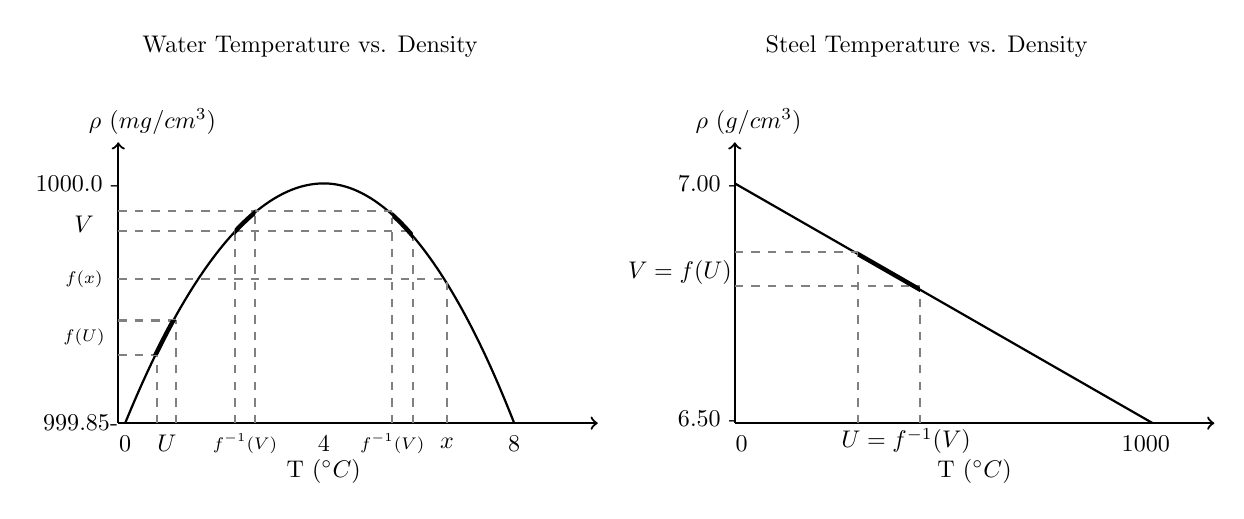
\begin{tikzpicture}[thick,scale=0.87, every node/.style={scale=0.87}]
		
		\draw[thick,->] (-1,3) -- (6,3);
		\draw[thick,->] (-1,3) -- (-1,7.1);
		
		\node at (-0.5,7.4) {$\rho$ ($mg/cm^3$)};
		\node at (2,2.3) {T ($^\circ C$)};
		
		\node at (2,2.7) {4};
		\node at (4.78,2.7) {8};
		\node at (-0.9,2.7) {0};
		
		\node at (-1.6,6.5) {1000.0 -};
		\node at (-1.55,3.01) {999.85-};
		
		
		\draw (2,6.5) parabola (4.78,3);
		\draw (2,6.5) parabola (-0.9,3);
		
		\draw[gray,thick,dashed] (-1,5.1) -- (3.8,5.1);
		
		\draw[gray,thick,dashed] (3.8,3) -- (3.8,5.1);
		
		\node at (3.8,2.7) {$x$};
		\node at (-1.5,5.1) {$\scriptstyle f(x)$};
		
		
		\draw[gray,thick,dashed] (-1,4.5) -- (-0.16,4.5);
		\draw[gray,thick,dashed] (-1,4) -- (-0.43,4);
		
		\draw[gray,thick,dashed] (-0.16,3) -- (-0.16,4.5);
		\draw[gray,thick,dashed] (-0.43,3) -- (-0.43,4);
		
		\node at (-0.29,2.7) {$U$};
		\node at (-1.5,4.25) {$\scriptstyle f(U)$};
		
		
		\draw[gray,thick,dashed] (0.7,3) -- (0.7,5.8);
		\draw[gray,thick,dashed] (1,3) -- (1,6.1);
		
		\draw[gray,thick,dashed] (-1,5.8) -- (3.25,5.8);
		\draw[gray,thick,dashed] (-1,6.1) -- (3,6.1);
		
		\draw[gray,thick,dashed] (3,3) -- (3,6);
		\draw[gray,thick,dashed] (3.3,3) -- (3.3,5.7);
		
		\node at (0.85,2.7) {$\scriptstyle f^{-1}(V)$};
		\node at (3.0,2.7) {$\scriptstyle f^{-1}(V)$};
		\node at (-1.5,5.9) {$V$};
		
		\begin{scope}
			\clip (-0.5,4) rectangle (0.2,4.5);
			\draw[black, ultra thick] (2,6.5) parabola (-0.9,3);
		\end{scope}
		
		\begin{scope}
			\clip (0.7,5.2) rectangle (1,6.5);
			\draw[black, ultra thick] (2,6.5) parabola (-0.9,3);
		\end{scope}
		
		\begin{scope}
			\clip (3,5) rectangle (3.3,6.3);
			\draw[black, ultra thick] (2,6.5) parabola (4.78,3);
		\end{scope}
		
		
		\draw[thick,->] (8,3) -- (15,3);
		\draw[thick,->] (8,3) -- (8,7.1);
		
		\node at (11.5,2.3) {T ($^\circ C$)};
		\node at (8.2,7.4) {$\rho$ ($g/cm^3$)};
		
		\draw (8,6.5) -- (14.1,3);
		
		\node at (7.6,6.5) {7.00 -};
		\node at (7.6,3.06) {6.50 -};
		\node at (14,2.7) {1000};
		\node at (8.1,2.7) {0};
		
		\draw[gray,thick,dashed] (8,5.5) -- (9.8,5.5);
		\draw[gray,thick,dashed] (8,5) -- (10.7,5);
		
		\draw[gray,thick,dashed] (9.8,3) -- (9.8,5.5);
		\draw[gray,thick,dashed] (10.7,3) -- (10.7,4.9);
		
		\begin{scope}
			\clip (9.8,4.5) rectangle (10.7,5.5);
			\draw[black, ultra thick] (8,6.5) -- (14.1,3) ;
		\end{scope}
		
		
		\node at (10.5,2.74) {$U=f^{-1}(V)$};
		\node at (7.2,5.2) {$V=f(U)$};
		
		
		\node at (1.8,8.5) {Water Temperature vs. Density};
		\node at (10.8,8.5) {Steel Temperature vs. Density};
	\end{tikzpicture}
\end{center}


It should be evident that we cannot impose inference relationships between any two domains: it's something that the domains allow or not. The domains for the temperature of two different mercury columns are in general not related: testing the value of one does not tell us anything about the other. The topologies of the two domains, however, are going to be the same because we'll have the same possible values and the same way to experimentally test them. Equivalence between experimental domains is a much stronger relationship than equivalence of the natural topology. It carries enough of the semantic to be able to tell what spaces are truly scientifically equivalent.

Let's continue with our example. We can re-express a relationship between domains in terms of causal relationship between the two domains. If $x$ is the value of temperature of the mercury column (i.e. a possibility for $\edomain_X$) and $y$ is the height of the mercury column (i.e. a possibility for $\edomain_Y$), then we can write $y=f(x)$ since the height is determined by the temperature.

Note that the direction of the causal relationship is the opposite of the inference. $X$ causes $Y$ and from $\edomain_Y$ we can infer $\edomain_X$ . Chains of events are in terms of possibilities and start with the cause and end with the effect. Chains of inferences are in terms of verifiable statements and start with the result and end with the origin.

The other directions do not work in general. Even if we know the final possibility, we may not be able to reconstruct the initial possibility: if the water density is exactly 999.9 kg/$m^3$, the temperature could be either 0.52 or 7.6 Celsius because density peaks at 4 Celsius. For the same reason, a measurement of the cause is not always equivalent to a measurement of the effect: verifying that \statement{the water temperature is between 0 and 0.52 Celsius} will mean that \statement{the water density is between 999.8 and 999.9 kg/$m^3$} but not the other way around. Because of the peak in density, the statement about the temperature tells us more (i.e. it is narrower) than the statement about the density and therefore they are not equivalent. That is: we can learn more about the temperature by measuring it directly than indirectly through the density.

Another important consideration is that, in order to be consistent, the function $y=f(x)$ has to be continuous. The general idea is the following: if we say that we can only measure both the temperature and height of a mercury column with finite precision, we have to make sure that we can use the causal relationship for inference. Therefore a finite precision measurement of height will correspond to a finite precision measurement of temperature. This means a small change in height has to correspond to a small change in temperature: the function is continuous.

More precisely, consider the verifiable statement $\stmt_Y=$\statement{the height of the mercury column is between 24 and 25 millimeters}. The height of the mercury column $y$ is within the verifiable set $U(\stmt_Y) = (24, 25)$ millimeters. We can then infer that the temperature must be in the reverse image of the possible heights $f^{-1}(U_Y(\stmt_Y))=(24,25)$ Celsius. But this means that, indirectly, we have experimentally verified that $x$ is in $f^{-1}(U_Y(\stmt_Y))$. And if $\edomain_X$ is really the domain of the verifiable statements for the temperature, then it must contain one that matches \statement{the temperature of the mercury column is between 24 and 25 Celsius}. In other words, $f^{-1}(U_Y(\stmt_Y))$ must be a set in the topology of $X$ and the function is continuous.\footnote{In topology, continuity is defined in terms of the sets in the topology and not in terms of small changes as in analysis. When using the standard topology on real numbers, the two coincide but not in general.}

\begin{mathSection}
	\begin{defn}
		Let $(X, \mathsf{T}_X)$ and $(Y, \mathsf{T}_Y)$ be two topological spaces. A \textbf{continuous function} is a map $f: X \to Y$ such that given any verifiable set $U_Y \in \mathsf{T}_Y$ its reverse image $f^{-1}(U_Y) \in \mathsf{T}_X$ is a verifiable set. A \textbf{homeomorphism} is a continuous bijective map such that its inverse is also continuous.
	\end{defn}
	\begin{defn}
		A \textbf{causal relationship} between two experimental domains establishes that determining which possibility is true in the first domain also determines which possibility is true in the second. Formally, a causal relationship between two experimental domains $\edomain_X$ and $\edomain_Y$ is a function $f : X \to Y$ between the possibilities of the respective domains such that $x \narrower f(x)$ for all $x \in X$.
	\end{defn}
	\begin{coro}
		All causal relationships are continuous functions over the respective natural topologies.
	\end{coro}
	\begin{proof}
		Let $f : X \to Y$ be a causal relationship between $\edomain_X$ and $\edomain_Y$. Let $y \in Y$ be a possibility for $\edomain_Y$. Consider $f^{-1}(y)$: this is the set of all possibilities in $X$ that are compatible with $y$ which is, by definition, the theoretical set of $y$. Therefore we have $y \equiv \bigOR\limits_{x \in f^{-1}(y)} x$. Now consider a verifiable statement $\stmt_Y \in \edomain_Y$ and the associated verifiable set $U_Y(\stmt_Y) \subseteq Y$. We have $\stmt_Y \equiv \bigOR\limits_{y \in U_Y(\stmt_Y)} y \equiv \bigOR\limits_{y \in U_Y(\stmt_Y)} \bigOR\limits_{x \in f^{-1}(\{y\})} x \equiv \bigOR\limits_{x \in f^{-1}(U_Y(\stmt_Y))} x$. Given that $\stmt_Y$ is verifiable, $\bigOR\limits_{x \in f^{-1}(U_Y(\stmt_Y))} x$ is also verifiable because it is equivalent to a verifiable statement. Since $f^{-1}(U_Y(\stmt_Y))$ is the set of possibilities compatible with that statement, $f^{-1}(U_Y(\stmt_Y))$ must be a verifiable set and therefore $f^{-1}(U_Y(\stmt_Y)) \in \mathsf{T}_X$ must be in the natural topology of $\edomain_{X}$. Therefore $f$ is a continuous function over the respective natural topologies.
	\end{proof}
	\begin{coro}
		A causal relationship between two domains is unique if it exists.
	\end{coro}\label{pm-cd-causalRelationshipUniqueness}
	\begin{proof}
		Suppose $f_1 : X \to Y$ and $f_2 : X \to Y$ are two causal relationships. Let $x \in X$. We have $x \narrower f_1(x)$ and $x \narrower f_2(x)$. This means $f_1(x) \comp f_2(x)$. But these are two possibilities of the same domain, so they are either incompatible or are the same possibilities. Therefore $f_1(x) \equiv f_2(x)$ for all $x \in X$. The causal relationships are the same.
	\end{proof}
	\begin{thrm}[Experimental Relationship Theorem]\label{pm-cd-experimentalRelationshipTheorem}
		Inference and causal relationships are equivalent. More formally, let $\edomain_X$ and $\edomain_Y$ be two experimental domains. An inference relationship $\erel: \edomain_Y \to \edomain_X$ exists between them if and only if a causal relationship $f: X \to Y$ also exists.
	\end{thrm}
	\begin{proof}
		First we show that a causal relationship exists between the independent and the dependent domain. Suppose $\edomain_Y$ depends on $\edomain_X$. Given that for each statement in $\edomain_Y$ there exists an equivalent statement in $\edomain_X$, $\edomain_Y$ is effectively a subset of $\edomain_X$. Moreover, since the theoretical domains for both experimental domains are generated by completing under negation, the theoretical domain $\tdomain_Y$ will effectively be a subset of $\tdomain_X$. This means that a possibility $x \in \tdomain_X$, if true, will determine all the truth values of  all statements in $\tdomain_Y$, including its possibilities. Because one possibility of $Y$ must be true and because all possibilities are incompatible with each other, there must be one and only one possibility $y \in \tdomain_Y$ compatible with $x$. Therefore we can define $f : X \to Y$ the function that given a possibility $x \in X$ returns the only possibility $y=f(x) \broader x$ that is compatible with it.
		
		We still need to show that $f$ is continuous. Consider a verifiable statement $\stmt_Y \in \edomain_Y$. Let $U_Y(\stmt_Y) \in \mathsf{T}_Y$ be its verifiable set. Since $\edomain_Y$ depends on $\edomain_X$, we can find $\stmt_X \in \edomain_X$ such that $\stmt_X \equiv \stmt_Y$. Let $U_X(\stmt_X) \in \mathsf{T}_X$ be its verifiable set. This is also the set of all possibilities in $X$ that are compatible with $\stmt_Y$, which means $U_X(\stmt_X)$ contains all the possibilities that are compatible with a possibility in $U_Y(\stmt_Y)$. Since $f$ returns the only possibility in $Y$ compatible with a possibility in $X$, $f^{-1}(U_Y(\stmt_Y))$ will return all the possibilities in $X$ that are compatible with a possibility in $U_Y(\stmt_Y)$. That means $f^{-1}(U_Y(\stmt_Y)) = U_X(\stmt_X)$ and that $f^{-1}$ maps verifiable sets to verifiable sets. Therefore $f$ is continuous.
		
		Now we show that a causal relationship implies dependence between domains. Suppose we have a causal relationship $f: X \to Y$ between $\edomain_X$ and $\edomain_Y$. Let $y \in Y$ be a possibility for $\edomain_Y$. Consider  $f^{-1}(\{y\})$: this is the set of all possibilities in $X$ that are compatible with $y$ which is, by definition, the theoretical set of $y$. Therefore we have $y \equiv \bigOR\limits_{x \in f^{-1}(\{y\})} x$. Now consider a verifiable statement $\stmt_Y \in \edomain_Y$. We have $\stmt_Y \equiv \bigOR\limits_{y \in U_Y(\stmt_Y)} y \equiv \bigOR\limits_{y \in U_Y(\stmt_Y)} \bigOR\limits_{x \in f^{-1}(\{y\})} x \equiv \bigOR\limits_{x \in f^{-1}(U_Y(\stmt_Y))} x$. Because $f$ is continuous, the reverse image of a verifiable set is a verifiable set. Therefore there is an $\stmt_X \in \edomain_X$ such that $U_X(\stmt_X) = f^{-1}(U_Y(\stmt_Y))$. The two verifiable statements $\stmt_X \equiv \bigOR\limits_{x \in U_X(\stmt_X)} x \equiv \stmt_Y$ are equivalent. For each $\stmt_Y \in \edomain_Y$ we can find an equivalent $\stmt_X \in \edomain_X$ so $\edomain_Y$ depends on $\edomain_X$.
	\end{proof}
	
	\begin{coro}
		Two experimental domains $\edomain_{X}$ and $\edomain_{Y}$ are equivalent if and only if there exists a homeomorphism $f : X \to Y$ between the possibilities such that $x \equiv f(x)$.
	\end{coro}
	\begin{proof}
		Let $\edomain_{X}$ and $\edomain_{Y}$ be two equivalent experimental domains. Then we can find the causal relationship $f : X \to Y$ and $g : Y \to X$. We have $x \narrower f(x) \narrower g(f(x))$. Since $g(f(x)) \in X$ is a possibility, and since $x$ is the only possibility compatible with itself, we must have $x \equiv g(f(x))$. Therefore $g$ is the inverse of $f$ and it is continuous. Therefore $f$ is a homeomorphism. We also have $x \narrower f(x) \narrower x$, therefore $f(x) \equiv x$.
		
		Now let $f : X \to Y$ be a homeomorphism between the possibilities of $\edomain_{X}$ and $\edomain_{Y}$ such that $x \equiv f(x)$. Then $f$ is a causal relationship and $\edomain_{Y}$ depends on $\edomain_{X}$. Let $g$ be the inverse of $f$, which is continuous since $f$ is a homeomorphism. We have $y \equiv f(g(y)) \equiv g(y)$. Then $g$ is also a causal relationship and $\edomain_{X}$ depends on $\edomain_{Y}$. Therefore $\edomain_{X} \equiv \edomain_{Y}$.
	\end{proof}
\end{mathSection}

Since for each inference relationship we have a causal relationship and vice-versa, we will simply use the term \textbf{experimental relationship} to describe the link between the two domains.

We should stress that causal relationships and inference relationships are defined on spaces that have, in a sense, a different status in a physical theory. Inference relationships are defined on verifiable statements, on finite precision measurements, which are the objects that are directly defined experimentally. In this sense, inferences have a higher status as they are more directly related to experimental verification. However, the map $\erel : \edomain_Y \to \edomain_X$ is over-complicated and redundant precisely because it maps all possible finite precision measurements from one domain to the other. Conversely, the causal relationship $f : X \to Y$ is only defined on the possibilities, on the points, therefore there is no redundancy. However, the possibilities are not verifiable statements in general and are often the product of idealizations. In this sense, causal relationships have a lower status as they are only indirectly defined by experimental verification.

The perfect correspondence between causal and inference relationships is what rescues and justifies the predominant focus on causal relationships to describe experimental relationships: since studying one is mathematically the same as studying the other, why should we use the more complicated object? Therefore, while the inference relationship is more directly physically meaningful, the causal relationship is a much more convenient object to study and characterize. That is why, in the end, all relationships will be predominantly defined by a function over the possibilities.

We now turn our attention back to domain equivalence. We have seen that two experimental domains $\edomain_X$ and $\edomain_Y$ are equivalent if they consist of equivalent statements: if they allow a one to one correspondence that preserves the equivalence of their statements. This implies, for example, that the possibilities are also equivalent but there is more to it.

Suppose we define some type of operation on one domain. For example, on the experimental domain for the temperature of a mercury column we define an increase by one Celsius; or on the experimental domain for the amount of gasoline in a tank we define the sum of two possible amounts. These will correspond either to operations on the domain (e.g. $f : \edomain_X \to \edomain_X$) or on its possibilities (e.g. $+ : X \times X \to X$). But by doing so we are also defining them on all equivalent domains as well: in the end, they are made of equivalent statements. Therefore we are also defining an increase of the height of the mercury column and the sum of the monetary value of the gasoline.

This means that if we capture some physical feature using some mathematical structure on one domain, then all equivalent domains will inherit the same structure. Moreover, the causal relationship is a function that preserves that structure. If the possibilities of one domain form a vector space, then the possibilities of an equivalent domain form a vector space and the causal relationship is an invertible linear transformation. If the possibilities of one domain form a group, then the possibilities of an equivalent domain form a group and the causal relationship is an isomorphism.\footnote{Domain equivalence is an isomorphism in whatever category (e.g. topological space, group, vector space, ...) used to model the experimental domain.} As we'll see much later, this is fundamental since deterministic and reversible evolution means equivalence of the domains describing the past, present and future states. Therefore deterministic and reversible motion is not ``just" a one to one map.

\begin{mathSection}
	\begin{thrm}[Domain Equivalence is Isomorphism]\label{pm-cd-domainEquivalenceIsIsomorphism}
		Let $\edomain_Y \equiv \edomain_X$ be two equivalent experimental domains. Suppose $\edomain_X$ is endowed with some mathematical structure. Then $\edomain_Y$ is also endowed with an equivalent structure and the experimental relationship preserves said structure.
	\end{thrm}
	\begin{proof}
		Since an experimental domain is really defined not on the statements themselves but on their equivalence classes, the mathematical structure will also be defined on the equivalence classes. But this means that a structure defined on $\edomain_X$ is also defined on $\edomain_Y$ since they contain the same equivalence classes. Therefore $\edomain_Y$ is also endowed with an equivalent structure.
		
		The experimental relationship can be either expressed as a map between possibilities $f : X \to Y$ or as a map between verifiable statements $\erel : \edomain_X \to \edomain_Y$. This means that the mathematical structure defined on $\edomain_Y$ can be transported to $\edomain_X$ using the experimental relationship. But since the mathematical structure defined on $\edomain_X$ already contains the mathematical structure defined on $\edomain_Y$, the transported mathematical structure has to be the same. That is, the experimental relationship must preserve the mathematical structure defined on $\edomain_X$.
	\end{proof}
\end{mathSection}

Note that the converse is not true: two domains that are endowed with the same mathematical structure are not necessarily equivalent. Consider two similarly constructed thermometers: their respective experimental domains are not equivalent since knowing something about one tells us nothing about the other. Yet, their natural topologies are equivalent because the way we can measure temperature for both is the same. One way to look at it is that the mathematical structures ``forget" the full equivalence between statements and only look at a particular aspect. Topological spaces capture how the possibilities are distinguished in terms of verifiable statements. Therefore, while the domains for temperature of two different thermometers are not equivalent, their natural topologies are equivalent because the way we characterize all possible measurements is the same (i.e. the value is within a finite precision interval). Similarly, the $\sigma$-algebra only cares about what statements can be associated to experimental tests. We'll see that, in some cases, Abelian groups will capture how distributions can be composed into other distributions, that non-Abelian groups will capture how transformations can be composed into other transformations, and so on.

\section{Combining domains}

In this section we want to understand what happens when we combine statements from different domains. For example, suppose we have the experimental domain for the pressure of an ideal gas and the experimental domain for its temperature. We can mix and match verifiable statements with conjunction and disjunction as in \statement{the pressure is between 1 and 1.1 KPa}$\AND$\statement{the temperature is between 20 and 21 C} creating a new domain. How can we characterize this combined experimental domain?

The main result of this section is that the possibilities of the combined domain depend on how compatible the verifiable statements of the domains are. In particular, if the verifiable statements are independent across domains (e.g. the horizontal and vertical position of an object), then the possibilities of the combined domain will be the Cartesian product of those for the individual domains. On the other hand, if the verifiable statements are incompatible across domains (e.g. plant identification and animal identification), then the possibilities for the combined domain will be the disjoint union of the possibilities of the individual domains.

Suppose $\edomain_X$ is the experimental domain generated by the two verifiable statements \statement{the patient is dead} and \statement{the patient is alive} and a second one $\edomain_Y$ generated by the two verifiable statements \statement{the patient is not in a coma} and \statement{the patient is in a coma}. The given verifiable statements also correspond to the possibilities for the respective domains.

We can construct the combined domain $\edomain_X \times \edomain_Y$ by taking all possible disjunctions and conjunctions. What are the possibilities for the new domain? Since by \ref{pm-vs-possibilitiesAreMinterms} the possibilities are minterms, we have the following cases to consider:
\begin{itemize}
	\item \statement{the patient is alive} $\AND$ \statement{the patient is in a coma}
	\item \statement{the patient is alive} $\AND$ \statement{the patient is not in a coma}
	\item \statement{the patient is dead} $\AND$ \statement{the patient is in a coma}
	\item \statement{the patient is dead} $\AND$ \statement{the patient is not in a coma}
\end{itemize}
The third one is impossible: the patient cannot be dead and in a coma. Therefore the combined domain has only three possibilities. The possibilities of the combined domain are, in general, the subset of all possible combinations (i.e. the Cartesian product) of the possibilities of the domains we are combining, those that are not impossible.

\begin{mathSection}
	%TODO: Choose a different symbols for domain combination. Introduce somewhere "projections" as maps between domains. Show that domain combination is both the product and coproduct.
	
	\begin{defn}
		Let $\{\edomain_{X_i}\}_{i=1}^{\infty}$ be a countable set of experimental domains. The \textbf{combined experimental domain} $\edomain_{X} = \bigtimes\limits_{i=1}^{\infty} \edomain_{X_i}$ is the experimental domain generated from all statements in $\{\edomain_{X_i}\}_{i=1}^{\infty}$ by finite conjunction and countable disjunction.
	\end{defn}
	\begin{proof}
		We need to show that the combined experimental domain is indeed an experimental domain. It will contain the certainty and the impossibility since any of the original experimental domains contains them. It is closed under finite conjunction and countable disjunction by construction. To show that it has a countable basis, for each $i=1..\infty$ let $\basis_i \in \edomain_{X_i}$ be a countable basis for the respective domain. Consider $\basis=\bigcup\limits_{i=1}^\infty \basis_i$. From this set we can generate any $\edomain_{X_i}$ and therefore we can also generate all of $\edomain_{X}$. $\basis$ is a basis and it is countable since it is the union of a countable set of countable elements. Note that it is precisely because the basis needs to remain countable that we cannot extend the operation to an uncountable set of domains.
	\end{proof}
	
	\begin{prop}\label{pm-cd-combinedDomainPossibilities}
		The possibilities for a combined domain are a subset of the Cartesian product of the possibilities for the individual domains. Formally, let $\{\edomain_{X_i}\}_{i=1}^{\infty}$ be a countable set of experimental domains and $\{X_i\}_{i=1}^{\infty}$ their respective possibilities. Let $X$ be the set of possibilities for the combined domain $\edomain_{X} = \bigtimes\limits_{i=1}^{\infty} \edomain_{X_i}$.  Then $X = \{ x = \bigAND\limits_{i=1}^{\infty} x_i \, | \, \{x_i\}_{i=1}^{\infty} \in \bigtimes\limits_{i=1}^{\infty} X_i, \, x \nequiv \impossibility \}$.
	\end{prop}   
	\begin{proof}
		A possibility $x$ of the combined domain is a minterm of a basis $\basis \subseteq \edomain_{X}$. Since we can choose $\basis=\bigcup\limits_{i=1}^\infty \basis_i$ where $\basis_i \subseteq \edomain_{X_i}$ is a countable basis for each domain, $x$ is the conjunction $x \equiv \bigAND\limits_{i=1}^{\infty}x_i$ of minterms $x_i$ of $\basis_i$. Since $x$ is a possibility, it is not impossible and therefore none of the $x_i$ can be impossible. Since each $x_i$ is a minterm of the respective basis $\basis_i$ that is not impossible, it is a possibility by \ref{pm-vs-possibilitiesAreMinterms}. Therefore a possibility $x$ of the combined domain is the conjunction of the possibilities $x_i$ of the original domains that is not impossible.
	\end{proof}
	
	\begin{prop}
		Let $\{\edomain_{X_i}\}_{i=1}^{\infty}$ be a countable set of incomplete experimental domains and $\edomain_X$ their combined experimental domain. Let $\{\resPoss_i\}_{i=1}^{\infty}$ be  the residual possibility of each respective domain. Let $\resPoss = \bigAND\limits_{i=1}^{\infty} \resPoss_i$. The combined domain $\edomain_X$ is incomplete if and only if $\resPoss \nequiv \impossibility$ in which case $\resPoss$ is the residual possibility.
	\end{prop}
	
	\begin{proof}
		For each domain, the residual possibility is the conjunction of the negation of its basis. Therefore we have $\resPoss \equiv \bigAND\limits_{\stmt[e] \in \basis} \NOT \stmt[e] \equiv \bigAND\limits_{i=1}^{\infty} \bigAND\limits_{\stmt[e] \in \basis_i} \NOT \stmt[e] \equiv \bigAND\limits_{i=1}^{\infty} \resPoss_i$. If $\resPoss \nequiv \impossibility$ then it is the residual possibility.
	\end{proof}
	
	\begin{coro}
		The residual possibility of the combined domain is narrower than the ones of the original domains. If one of the domains is complete then the combined domain is also complete.
	\end{coro}
	
	\begin{proof}
		Let $\resPoss$ be the residual possibility for the combined domain and $\resPoss_j$ the one for one of the original domains. We have $\resPoss_j \AND \resPoss \equiv \resPoss_j \AND \bigAND\limits_{i=1}^{\infty} \resPoss_i \equiv \bigAND\limits_{i=1}^{\infty} \resPoss_i \equiv \resPoss$. Therefore, by \ref{pm-vs-narrownessProperties} $\resPoss \narrower \resPoss_j$.
		
		Suppose that one of the original domains $\edomain_{X_j}$ is complete. Then the conjunction of the negation of its basis $\resPoss_j$ is an impossibility. This means the conjunction of the negation of the basis of the combined domain $\resPoss$ is also an impossibility and the combined domain is complete.
	\end{proof}
\end{mathSection}

\subsection{Independent domains}

A special case is when combining two independent domains. For example, the domain for the pressure and the domain for the volume of an ideal gas are independent because a measurement on one tells us nothing about the other. Similarly, the domain for the shape and the domain for the color of an object are independent. In these cases, we can have any combination of possibilities: any pressure with any volume or any color with any shape.

In terms of topology, the possibilities of the combined domain are the Cartesian product of the possibilities of the original domains and their natural topology is the product topology.\footnote{Note that the topology is quite naturally the product topology and not the box topology. The box topology would require countable conjunction and is therefore discarded. The fact that the correct topology is the one most natural to define confirms again the appropriateness of our framework.}

\begin{figure}[h]
	\centering
	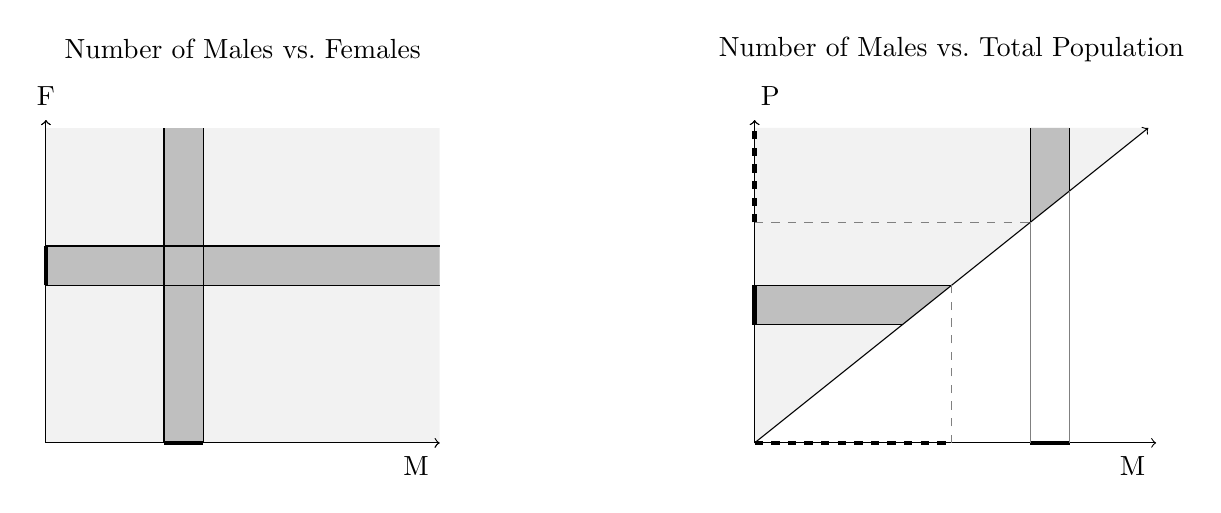
\begin{tikzpicture}
		\draw[->] (-1,3) -- (4,3);
		\draw[->] (-1,3) -- (-1,7.1);
		
		\node at (-1,7.4) {F};
		\node at (3.7,2.7) {M};
		
		\begin{scope}
			\clip (-1,3) rectangle (4,7);
			\fill[gray!10!white] (-1,3) rectangle (4,7);
		\end{scope}
		
		\begin{scope}
			\clip (-1,5) rectangle (4,5.5);
			\fill[gray!50!white] (-1,5) rectangle (4,5.5);
		\end{scope}
		
		\begin{scope}
			\clip (0.5,3) rectangle (1,7);
			\fill[gray!50!white] (0.5,3) rectangle (1,7);
		\end{scope}
		
		\begin{scope}
			\clip (0.5,5) rectangle (1,5.5);
			\fill[gray!50!white] (0.5,5) rectangle (1,5.5);
		\end{scope}
		
		\draw[black] (-1,5)--(4,5);
		\draw[black] (-1,5.5)--(4,5.5);
		
		\draw[black] (0.5,3) -- (0.5,7);
		\draw[black] (1,3) -- (1,7);
		
		
		\draw[->] (-1,3) -- (4,3);
		\draw[->] (-1,3) -- (-1,7.1);
		
		
		\draw[->] (8,3) -- (13.1,3);
		\draw[->] (8,3) -- (8,7.1);
		
		\draw[black,ultra thick] (-1,5) -- (-1,5.5);
		\draw[black,ultra thick] (0.5,3) -- (1,3);
		
		\node at (12.8,2.7) {M};
		\node at (8.2,7.4) {P};
		
		\begin{scope}
			\clip (8,3) -- (8,4.5) -- (9.89,4.5) -- (8,3);
			\fill[gray!10!white] (8,3) -- (8,4.5) -- (9.89,4.5) -- (8,3);
		\end{scope}
		\begin{scope}
			\clip (8,5) -- (10.5,5) -- (13,7) -- (8,7) -- (8,5);
			\fill[gray!10!white] (8,5) -- (10.5,5) -- (13,7) -- (8,7) -- (8,5);
		\end{scope}
		
		\begin{scope}
			\clip (8,4.5) -- (8,5) -- (10.5,5) -- (9.8,4.5) -- (8,4.5);
			\fill[gray!10!white] (8,4.5) -- (8,5) -- (10.5,5) -- (9.8,4.5) -- (8,4.5);
		\end{scope}
		
		\draw[->] (8,3) -- (8,7.1);
		
		
		\begin{scope}
			\clip (8,4.5) -- (8,5) -- (10.5,5) -- (9.89,4.5) -- (8,4.5);
			\fill[gray!50!white] (8,4.5) -- (8,5) -- (10.5,5) -- (9.89,4.5) -- (8,4.5);
		\end{scope}
		\begin{scope}
			\clip (11.5,5.8) -- (11.5,7) -- (12,7) -- (12,6.2) -- (11.5,5.8);
			\fill[gray!50!white] (11.5,5.8) -- (11.5,7) -- (12,7) -- (12,6.2) -- (11.5,5.8);
		\end{scope}
		
		\draw[->] (8,3) -- (13,7);
		
		\draw[black] (8,4.5) -- (9.89,4.5);
		\draw[black] (8,5) -- (10.5,5);	
		
		\draw[black, ultra thick, dashed] (8,3) -- (10.5,3);	
		\draw[black,ultra thick] (8,4.5) -- (8,5);
		
		\draw[gray,dashed] (10.5,3) -- (10.5,5);
		
		\draw[gray,dashed] (8,5.8) -- (11.5,5.8);
		
		\draw[black,ultra thick] (11.5,3) -- (12,3);
		\draw[black,ultra thick,dashed] (8,5.8) -- (8,7);
		
		\draw[gray] (11.5,3) -- (11.5,5.8);
		\draw[gray] (12,3) -- (12,6.2); 
		\draw[black] (11.5,5.8) -- (11.5,7);
		\draw[black] (12,6.2) -- (12,7);
		
		
		\node at (1.5,8) {Number of Males vs.~Females};
		\node at (10.5,8) { Number of Males vs.~Total Population};
	\end{tikzpicture}
	\caption{Domain independence and projections. Given a population, the number of male and female members form independent domains: knowing something about one value tells us nothing about the other. Pictorially, a constraint on one side gives us a vertical or horizontal band, which projected on the other axis, gives us the full axis (i.e.~the certainty). On the other hand, the total population and the number of males are not independent domains: given the total population, the number of males cannot exceed that number; given the number of males, the total population cannot be lower than that number. Pictorially, we see that the combined domain does not span the whole plane. A constraint on one domain gives us, when projected, a constraint on the other domain.} \label{pm-cd-fig-relationships}
\end{figure}



\begin{mathSection}
	\begin{defn}
		The experimental domains of a countable set $\{\edomain_{X_i}\}_{i=1}^{\infty}$ are \textbf{independent} if taking one verifiable statement $\stmt_i \in \edomain_{X_i}$ from each domain always gives an independent set of statements.
	\end{defn}
	\begin{prop}
		Let $\{\edomain_{X_i}\}_{i=1}^{\infty}$ be a countable set of independent experimental domains and $X_i$ their respective possibilities. The set of possibilities $X$ of the combined experimental domain $\bigtimes\limits_{i=1}^{\infty} \edomain_{X_i}$ consists of all the possible conjunctions of the possibilities of each domain. That is: $X = \{ \bigAND\limits_{i=1}^{\infty} x_i \, | \, x_i \in X_i \}$. Notationally, we write $\edomain_X=\edomain_{\bigtimes\limits_{i=1}^{\infty} X_i}$.
	\end{prop}
	\begin{proof}
		A possibility $x \equiv \bigAND\limits_{i=1}^{\infty}x_i$ for the combined domain is the conjunction of possibilities of each individual domain by \ref{pm-cd-combinedDomainPossibilities}. Since the domains are independent and since possibilities are neither certainties nor impossibilities, by \ref{pm-vs-defStatementIndependence} there exists an assignment $a \in \pAss$ such that $a(x_i) = \TRUE$ for all $i=1..\infty$ and therefore $a(x)=\TRUE$. That is, each conjunction $x=\bigAND\limits_{i=1}^{\infty}x_i$ is not impossible and therefore is a possibility.
	\end{proof}
	\begin{defn}
		Let $\{(X_i, \mathsf{T}_i)\}_{i=1}^{\infty}$ be a countable set of topological spaces. Let $X=\bigtimes\limits_{i=1}^{\infty} X_i$ be the Cartesian product of the points. Let $\mathcal{B}$ be the collection of sets of the form $\bigtimes\limits_{i=1}^{\infty} U_{i}$, with $U_i \in \mathsf{T}_i$ and $U_i \neq X_i$ only finitely many times. The topology generated by $\mathcal{B}$ is called the \textbf{product topology}.
	\end{defn}
	\begin{prop}
		Let $\{\edomain_{X_i}\}_{i=1}^{\infty}$ be a countable set of independent experimental domains. The natural topology for the possibilities of the combined experimental domain $\edomain_{\bigtimes\limits_{i=1}^{\infty} X_i}$ is the product topology of the natural topology for the possibilities of each domain.
	\end{prop}
	\begin{proof}
		Let $U_i : \edomain_{X_i} \to \mathsf{T}_{X_i}$ be the map from a verifiable statement of a domain to its verifiable set in the respective topology. Let $U : \edomain_{X} \to \mathsf{T}_X$ be the same map for the combined domain. Let $\stmt_i \in \edomain_{X_i}$ be a verifiable statement from a particular domain and $U_i(\stmt_i)$ its verifiable set in that domain. Since we also have $\stmt_i \in \edomain_{X}$, the statement is also associated with the verifiable set $U(\stmt_i)$ in the combined domain. Because the domains are independent, every possibility in $U_i(\stmt_i)$ is compatible with any possibility $x_j \in X_j$ for all $j \neq i$. This means that $U(\stmt_i)=X_1\times ... \times X_{i-1} \times U_i(\stmt_i) \times X_{i+1} \times ...$ . Given that a verifiable statement in the combined domain can be generated using finite conjunction and countable disjunction from the verifiable statements of the independent domains, the topology of the combined space can be generated by all sets of the form $\bigtimes\limits_{i=1}^{\infty} U_{i}$, with $U_i \in \mathsf{T}_i$ and $U_i \neq X_i$ only once. Using finite conjunction, this includes those sets where $U_i \neq X_i$ finitely many times. The natural topology of the combined domain is the product topology by definition.
	\end{proof}
\end{mathSection}

\subsection{Dependent domains}

Another special case is combining a domain $\edomain_X$ with another $\edomain_Y \subseteq \edomain_X$ that is dependent on it. For example, combining the domain for the temperature of a mercury column with the domain for its height. Since the height can be determined by the temperature, no new possibilities are added. The combined domain is equivalent to the independent domain $\edomain_X$ since all the verifiable statements in $\edomain_Y$ have equivalents in it.

\begin{mathSection}
	\begin{prop}
		Let $\edomain_X$ and $\edomain_Y$ be two experimental domains such that $\edomain_Y \subseteq \edomain_X$ depends on the first. Then $\edomain_X \times \edomain_Y \equiv \edomain_X$.
	\end{prop}
	\begin{proof}
		Since $\edomain_Y$ is dependent on $\edomain_X$, any statement in $\edomain_Y$ is equivalent to one in $\edomain_X$. Therefore no statement can be generated from them that is not equivalent to one already contained in $\edomain_X$. Therefore $\edomain_X \times \edomain_Y$ is equivalent to $\edomain_X$. 
	\end{proof}
	\begin{coro}
		Let $\edomain_X$ and $\edomain_Y$ be two experimental domains such that $\edomain_Y \subseteq \edomain_X$ depends on the first. The possibilities of $\edomain_X \times \edomain_Y$ are the possibilities of $\edomain_X$.
	\end{coro}
	\begin{proof}
		The possibilities of $\edomain_X \times \edomain_Y$ are the possibilities of $\edomain_X$ since they are equivalent domains. To be consistent with \ref{pm-cd-combinedDomainPossibilities}, we additionally show that they are also the subset of the Cartesian product. Let $f : X \to Y$ be the causal relationship between the domains, let $x$ and $y$ be two possibilities of the respective domains. We have $x \AND y \nequiv \impossibility$ if and only if $y = f(x)$, so the possibilities of $\edomain_X \times \edomain_Y$ are $x \AND f(x)$ for all $x \in X$. We also have $x \AND f(x) \equiv x$ since $x \narrower f(x)$.
	\end{proof}
\end{mathSection}


\subsection{Incompatible domains}

The last special case we consider is when the domains are incompatible, that is all verifiable statements of one are incompatible with the verifiable statements of the others. This is one case where the residual possibility behaves differently from all the others.\footnote{In fact, this is what prompted us to introduce the residual possibility.} Suppose $\edomain_X$ is the domain to classify a particular specimen as an animal and $\edomain_Y$ is the domain to classify it as a plant. If we take a verifiable statement from the first, such as \statement{that specimen has fur}, then it will be incompatible with a verifiable statement from the other, such as \statement{that specimen has lobed leaves}. The only way we can combine the possibilities is to take an established possibility of one (e.g. \statement{this specimen is a cat}) and combine it with the residual possibility of the other (e.g. \statement{this specimen is not a plant}). In other words, the combined possibilities are the union of the possibilities of the two domains (e.g. all possible plants and all possible animals).

In terms of the topology, the established possibilities of the combined domain are the disjoint union of the established possibilities of the original domains and their natural topology is the disjoint union topology (or co-product topology). 

\begin{mathSection}
	\begin{defn}
		Two experimental domains $\edomain_X$ and $\edomain_Y$ are \textbf{incompatible} if all verifiable statements in one are incompatible with all verifiable statements of the other. Formally, $\stmt_X \ncomp \stmt_Y$ for each pair of verifiable statements $\stmt_X \in \edomain_X$ and $\stmt_Y \in \edomain_Y$.
	\end{defn}
	\begin{coro}
		Let $\edomain_X$ and $\edomain_Y$ be two incompatible experimental domains. Then they must be incomplete and admit a residual possibility.
	\end{coro}
	\begin{proof}
		Let $\basis_X$ and $\basis_Y$ be a countable basis for the respective domain. Since we have $\stmt[e]_X \ncomp \stmt[e]_Y$ for all choices of $\stmt[e]_X \in \basis_X$ and $\stmt[e]_Y \in \basis_Y$, we also must have $\bigOR\limits_{\stmt[e]_X \in \basis_X} \stmt[e]_X \ncomp \bigOR\limits_{\stmt[e]_Y \in \basis_Y} \stmt[e]_Y$. Therefore $\bigOR\limits_{\stmt[e]_X \in \basis_X} \stmt[e]_X \nequiv \certainty$. Which means the residual possibility $\mathring{x} = \bigAND\limits_{\stmt[e]_X \in \basis_X} \NOT\stmt[e]_X = \NOT \bigOR\limits_{\stmt[e]_X \in \basis_X} \stmt[e]_X \nequiv \impossibility$. Therefore $\edomain_X$ is not complete and, by symmetry, neither is $\edomain_Y$.
	\end{proof}
	\begin{prop}
		Let $\{\edomain_{X_i}\}_{i=1}^{\infty}$ be a countable set of experimental domains pair-wise incompatible and $\dot{X}_i$ their respective established possibilities. The set of established possibilities $\dot{X}$ of the combined experimental domain $\bigtimes\limits_{i=1}^{\infty} \edomain_{X_i}$ consists of the disjoint union of the possibilities of each domain. That is: $\dot{X} = \coprod\limits_{i=1}^{\infty} \dot{X}_i = \bigcup\limits_{i=1}^{\infty} \dot{X}_i$ as $\dot{X}_i \cap \dot{X}_j = \emptyset$ for all $i,j \geq 1$ and $i \neq j$. Notationally, we write $\edomain_X=\edomain_{\coprod\limits_{i=1}^{\infty} X_i}$.
	\end{prop}
	\begin{proof}
		Consider two incompatible domains $\edomain_X$ and $\edomain_Y$. Let $\dot{x} \in X$ and $\dot{y} \in Y$ be two established possibilities. Then they both correspond to a minterm of the respective basis where at least one element is taken without negation. This also means that their conjunction will include the conjunction of one element of each of the basis. Since the elements of one basis are incompatible with the elements of the other, we have $\dot{x} \ncomp \dot{y}$.
		
		Now let $\dot{x} \in X$ be an established possibility, $\mathring{y} \in Y$ the residual and $\dot{Y} = Y \setminus \{\mathring{y}\}$ the established possibilities. We have $\dot{x} \equiv \dot{x} \AND \certainty \equiv \dot{x} \AND \bigOR\limits_{y \in Y} y \equiv \dot{x} \AND (\bigOR\limits_{\dot{y} \in \dot{Y}} \dot{y} \OR \mathring{y}) \equiv \bigOR\limits_{\dot{y} \in \dot{Y}} (\dot{x} \AND \dot{y}) \OR (\dot{x} \AND \mathring{y}) \equiv \impossibility \OR (\dot{x} \AND \mathring{y}) \equiv \dot{x} \AND \mathring{y}$. By symmetry, $\dot{y} \equiv \mathring{x} \AND \dot{y}$.
		
		To conclude, let $\mathring{x} \in X$ and $\mathring{y} \in Y$ be the two residual possibilities. The conjunction $\mathring{x} \AND \mathring{y}$ corresponds to a minterm where all the elements of the basis are negated. Therefore $\mathring{x} \AND \mathring{y}$ is the residual possibility of the combined domain, if it is not impossible. 
		
		Generalizing to a countable set of incompatible domains, the conjunction of all the residual possibilities $\mathring{x}= \bigAND_{i=1}^{\infty} \mathring{x}_i$ is the residual possibility of the combined domain, if it is not impossible. The only other conjunctions of the form $x= \bigAND_{i=1}^{\infty} x_i$ with $x_i \in X_i$ for all $i \geq 1$ that are not impossible are those where only one element is not a residual possibility. Those correspond to the established possibilities. But each of those conjunctions will be equivalent to the only element that is not a residual possibility. Therefore each established possibility of the combined domain is equivalent to an established possibility of one of the original domains: $\dot{X} = \bigcup\limits_{i=1}^{\infty} \dot{X}_i$. Given that the established possibilities of two incompatible domains are incompatible and therefore different, we have $\dot{X}_i \cap \dot{X}_j = \emptyset$ for all $i,j \geq 1$ and $i \neq j$. The established possibilities of the combined domains are the disjoint union of the established possibilities of the individual domains.
	\end{proof}
	
	\begin{defn}
		Let $\{(X_i, \mathsf{T}_i)\}_{i=1}^{\infty}$ be a countable set of topological spaces. Let $X=\coprod\limits_{i=1}^{\infty} X_i$ be the disjoint union of the points. The \textbf{disjoint union topology} $\mathsf{T}$ is the topology for which $U \in \mathsf{T}$ if and only if $U \cap X_i \in \mathsf{T}_i$ for all $i \geq 1$.
	\end{defn}
	
	\begin{prop}\label{pm-cd-disjointUnionTopologyIsClosure}
		The disjoint union topology is generated by closing the topologies of the initial spaces under disjoint union.
	\end{prop}
	\begin{proof}
		First we show that all disjoint unions of verifiable sets are part of the disjoint union topology. Let $\{(X_i, \mathsf{T}_i)\}_{i=1}^{\infty}$ be a countable set of topological spaces and $(X, \mathsf{T})$ their disjoint union with the disjoint union topology. Any disjoint union of verifiable sets can be put in the form $U=\coprod\limits_{i=1}^{\infty} U_i$ with $U_i \in \mathsf{T}_i$ for all $i \geq 1$. We have $U \cap X_i = \coprod\limits_{i=j}^{\infty} U_j \cap X_i = U_i$ for all $i \geq 1$. Therefore $U \in \mathsf{T}$ by definition.
		
		Now we show that any set in the disjoint union topology is the disjoint union of verifiable sets of the individual topologies. Let $U \in \mathsf{T}$. Since $U \subseteq X$ and $X$ is the disjoint union for all $X_i$, we can write $U=\coprod\limits_{i=1}^{\infty} U_i$. As before $U \cap X_i = U_i$ for all $i \geq 1$ and, since $U \cap X_i \in \mathsf{T}_i$ for all $i \geq 1$ by definition of the disjoint union topology, $U_i \in \mathsf{T}_i$ for all $i \geq 1$. Therefore any $U \in \mathsf{T}$ is the disjoint union of verifiable sets.
		
		This also shows that the disjoint union topology is a topology since it is closed under arbitrary union by definition, it is closed under finite intersection within each topology and it is closed under finite intersection across topologies since their intersection is always the empty set.
	\end{proof}
	
	\begin{prop}
		Let $\{\edomain_{X_i}\}_{i=1}^{\infty}$ be a countable set of pair-wise incompatible domains. The natural topology for the established possibilities of the combined experimental domain $\edomain_{\coprod\limits_{i=1}^{\infty} X_i}$ is the disjoint union topology of the natural topology for the established possibilities of each domain.
	\end{prop}
	\begin{proof}
		Given that the domains are incompatible, they are also incomplete. The only statement in each domain $\edomain_{X_i}$ compatible with the respective residual possibility $\mathring{x}_i$ will be the certainty $\certainty$. This means the natural topology restricted to the established possibilities contains all the verifiable sets associated to the impossibilities and to all verifiable statements. This will also be true for the combined domain $\edomain_{\coprod\limits_{i=1}^{\infty} X_i}$, if it is incomplete. If it is complete, then the established possibilities are the full possibilities and their natural topology coincides. Note that all verifiable statements in the combined domain can be generated from the verifiable statements of the individual domains. Also note that the conjunction between the different domains is an impossibility and therefore does not yield a new statement. Therefore all the statements whose verifiable sets form the topology on the established possibilities on the combined domain can be generated by the disjunction of all the statements whose verifiable sets form  the topology on the established possibilities on the individual domains. Therefore the topology of the combined space is simply closing the individual topologies under the disjoint union. The topology of the combined space is therefore the disjoint union topology by \ref{pm-cd-disjointUnionTopologyIsClosure}
	\end{proof}
\end{mathSection}

For topologies, as well as for other mathematical structures, we can choose between two types of products. If we have two one dimensional euclidean spaces we can decide whether to take their product (i.e. the plane) or their co-product (i.e. the disjoint union of the two lines). For experimental domains we do not choose: it is what it is. There is no way to combine the two experimental domains for temperature and height of the same mercury column and get the Cartesian product of their possibilities. Though combining two independent domains mimics the categorical product and combining two incompatible domains mimics the categorical co-product, it is the semantic (and ultimately physical) relationship between them that decides which product we have. This is another case where the mathematical structures ``forget" the full equivalence. The topology only captures how the temperature and height can be measured, and not whether they are independent, dependent or incompatible. That information lies outside of the topology and therefore needs to be added by choosing the correct combination.

\section{Experimental domain for experimental relationships}

Now that we have seen how to describe relationships between domains, we should ask: are experimental relationships themselves something we can experimentally verify? We may know that there is a relationship between the temperature of a mercury column and its height, but how can we confirm experimentally which one it is?

The main result of this section is to show that, given two related experimental domains, we can always mathematically construct from them another experimental domain for which the possibilities are continuous functions between the possibilities of the original domains. This means that, since we can recursively create relationship domains about relationship domains, the universe of discourse of our mathematical framework is closed. Yet, the availability of the experimental tests (i.e. whether the statements we construct are actually verifiable) is not guaranteed.

First of all we have to clarify within our framework what it means to experimentally verify a relationship. Suppose $\edomain_X$ is the domain for the state of a light switch, up or down being the two possibilities, and $\edomain_Y$ is the domain for the state of the light, which can be on or off. Suppose we could have three cases: the one where the switch is wired correctly, up corresponding to on, the one where the switch is wired incorrectly, up corresponding to off, and the one where the switch is not actually wired to the light, the two domains are independent. Each of these cases is represented by a different set of logical relationships, a different set of possible assignments.

\begin{table}[h]
	\centering
	\begin{tabular}{c|c|c|c}
		\multicolumn{2}{c|}{X} & \multicolumn{2}{c}{Y} \\
		up & down & on & off \\
		\hline
		T & F & T & F \\
		F & T & F & T \\
	\end{tabular}
	\caption{Case 1: switch wired correctly to the light}
\end{table}

\begin{table}[h]
	\centering
	\begin{tabular}{c|c|c|c}
		\multicolumn{2}{c|}{X} & \multicolumn{2}{c}{Y} \\
		up & down & on & off \\
		\hline
		T & F & F & T \\
		F & T & T & F \\
	\end{tabular}
	\caption{Case 2: switch wired incorrectly to the light}
\end{table}

\begin{table}[h]
	\centering
	\begin{tabular}{c|c|c|c}
		\multicolumn{2}{c|}{X} & \multicolumn{2}{c}{Y} \\
		up & down & on & off \\
		\hline
		T & F & T & F \\
		T & F & F & T \\
		F & T & T & F \\
		F & T & F & T \\
	\end{tabular}
	\caption{Case 3: switch not wired to the light}
\end{table}

Each case, then, is a different model: a different logical context. To experimentally verify which model is the right one means verifying statements of the type \statement{it is possible for the switch to be up while the light is on}. This does not correspond to \statement{the switch is up} $\AND$ \statement{the light is on} but to \statement{the switch is up} $\comp$ \statement{the light is on}. These are statements about the table and they cannot be columns of the table itself. What we need to create is a metacontext, in which each line corresponds to one choice of model, to one context.

\begin{table}[h]
	\centering
	\begin{tabular}{r|c|c|c|c}
		& up $\comp$ on & down $\comp$ on & up $\comp$ off & down $\comp$ off \\
		\hline
		Case 1 & T & F & F & T \\
		Case 2 & F & T & T & F \\
		Case 3 & T & T & T & T \\
	\end{tabular}
	\caption{Possible assignments for the metacontext}
\end{table}

Each line will tell us what statements are compatible and given the truth values of the line we can reconstruct the model. The verifiable statements that distinguish between different models, therefore, live in this metacontext and so will the experimental domain for the relationships.

\begin{mathSection}
	\begin{defn}
		Let $\logCtx_1$ and $\logCtx_2$ be two logical contexts. Let $S_1 \subseteq \logCtx_1$ and $S_2 \subseteq \logCtx_2$ be sets of statements. We say $f : S_1 \to S_2$ is a \textbf{logic homomorphism} if it preserves the logical structure. That is:
		\begin{itemize}
			\item possible assignments on $S_2$ correspond to possible assignments on $S_1$: if $a_2 \in \pAss[S_2]$ then there exists $a_1 \in \pAss[S_1]$ such that $a_1(\stmt) = a_2(f(\stmt))$ for all $\stmt \in S_1$
			\item a verifiable statement of $S_1$ is mapped to a verifiable statement in $S_2$
		\end{itemize}
		Additionally, if there exists a logic homomorphism $g : S_2 \to S_1$ such that $f \circ g = \Id_{S_1}$ and $g \circ f = \Id_{S_2}$ then $f$ is a \textbf{logic isomorphism} and $g$ is the \textbf{inverse} of $f$. Two logic isomorphisms $f : S_1 \to S_2$ and $g : S_1 \to S_2$ are equivalent if $f(\stmt)\equiv g(\stmt)$ for all $\stmt \in S_1$.
	\end{defn}
	
	\begin{coro}\label{pm-cd-logicHomomorphismPreservesBooleanAlgebra}
		Let $h : S_1 \to S_2$ be a logic homomorphism, then for every $\hat{\stmt} \in S_1$, $\hat{S} \subseteq S_1$ and $f_\Bool : \Bool^{\hat{S}} \to \Bool$ such that $a_1(\hat{\stmt}) = f_\Bool(\{ a_1(\stmt) \}_{\stmt \in \hat{S}})$ for all $a_1 \in \pAss[S_1]$, then $a_2(h(\hat{\stmt})) = f_\Bool(\{ a_2(h(\stmt)) \}_{\stmt \in \hat{S}})$ for all $a_2 \in \pAss[S_2]$. In particular:
		\begin{itemize}
			\item $h(\NOT \stmt) \equiv \NOT h(\stmt)$ for all $\stmt \in S_1$
			\item $h(\bigAND_{\stmt \in S} \stmt) \equiv \bigAND_{\stmt \in S} h(\stmt)$ for all $S \subseteq S_1$
			\item $h(\bigOR_{\stmt \in S} \stmt) \equiv \bigOR_{\stmt \in S} h(\stmt)$ for all $S \subseteq S_1$
		\end{itemize}
	\end{coro}
	
	\begin{proof}
		If $a_1(\hat{\stmt}) = f_\Bool(\{ a_1(\stmt) \}_{\stmt \in \hat{S}})$ for all $a_1 \in \pAss[S_1]$ then, by the first property of logic homomorphisms, there is no $a_2 \in \pAss[S_2]$ such that $a_2(h(\hat{\stmt})) \neq f_\Bool(\{ a_2(h(\stmt)) \}_{\stmt \in \hat{S}})$. Therefore $a_2(h(\hat{\stmt})) = f_\Bool(\{ a_2(h(\stmt)) \}_{\stmt \in \hat{S}})$ for all $a_2 \in \pAss[S_2]$.
		
		In particular, since the relationship holds for any arbitrary $f_\Bool$, it will hold for negation, arbitrary conjunction and arbitrary disjunction.
	\end{proof}
	
	\begin{prop}
		Let $\logCtx_1$ and $\logCtx_2$ be two logical contexts. Let $S_1 \subseteq \logCtx_1$ and $S_2 \subseteq \logCtx_2$ be sets of statements and $f : S_1 \to S_2$ a logic homomorphism. Let $\bar{S}_1 \subseteq \logCtx_1$ and $\bar{S}_2 \subseteq \logCtx_2$ be the closure of $S_1$ and $S_2$ respectively under arbitrary conjunction, arbitrary disjunction and negation. Then if there exists a logic homomorphism $\bar{f} : \bar{S}_1 \to \bar{S}_2$ such that $\bar{f}(\stmt_1) \equiv f(\stmt_1)$ for all $\stmt_1 \in S_1$ it is unique.
	\end{prop}
	
	\begin{proof}
		Let $\tstmt_1 \in \bar{S}_1$ but $\tstmt_1 \notin S_1$. Then $\tstmt_1$ depends on $S_1$ through some $g_\Bool : \Bool^{S_1} \to \Bool$. Let $\bar{f}_1 : \bar{S}_1 \to \bar{S}_2$ and $\bar{f}_2 : \bar{S}_1 \to \bar{S}_2$ be two logic homomorphisms such that $\bar{f}_1(\stmt_1) \equiv \bar{f}_2(\stmt_1) \equiv f(\stmt_1)$ for all $\stmt_1 \in S_1$. Then by \ref{pm-cd-logicHomomorphismPreservesBooleanAlgebra} both $\bar{f}_1(\tstmt_1)$ and $\bar{f}_2(\tstmt_1)$ depend on $S_2$ through $g_\Bool$. This means that in every possible assignment $a \in \pAss[\bar{S}_2]$ we have $a(\bar{f}_1(\tstmt_1)) = a(\bar{f}_2(\tstmt_1))$  and therefore $\bar{f}_1(\tstmt_1) \equiv \bar{f}_2(\tstmt_1)$. Then $\bar{f}_1$ and $\bar{f}_2$ are equivalent.
	\end{proof}
	
	
	\begin{defn}
		Let $\edomain_X, \edomain_Y \subseteq \logCtx$ be two experimental domains. The \textbf{relationship metacontext}  $\logCtx_{C(X,Y)}$ between $\edomain_X$ and $\edomain_Y$ over $\{ \logCtx_i \}_{i \in I}$ is defined by following construction. Let $I$ be an index set. Let $\{ \logCtx_i \}_{i \in I}$ be an indexed set of logical contexts, let $\{ \edomain_{X_i} \}_{i \in I}$ and $\{ \edomain_{Y_i} \}_{i \in I}$ be two indexed sets of experimental domains such that $\edomain_{X_i}, \edomain_{Y_i} \subseteq \logCtx_i$ for all $i \in I$. Let $\{f_{i}\}_{i \in I}$ be a set of logic isomorphisms such that $f_{i} : \edomain_{X} \to \edomain_{X_i}$. Let $\{g_{i}\}_{i \in I}$ be a set of logic isomorphisms such that $g_{i} : \edomain_{Y} \to \edomain_{Y_i}$.
		
		Let $S$ be the set of ordered pairs of $\edomain_{X}$ and $\edomain_{Y}$ and \statement{$\stmt_x \comp \stmt_y$} be the notation of an element of $S$ for some $\stmt_x \in \edomain_{X}$ and $\stmt_y \in \edomain_{Y}$. For each $i \in I$, let $a_i \in \Bool^S$ be such that  $a_i(``\stmt_x \comp \stmt_y") = \TRUE$ if and only if $f_{i}(\stmt_x) \comp g_{i}(\stmt_y)$. Define $\pAss = \{ a_i \, | \, \forall i \in I \}$. Assume $a_i \neq a_j$ if $i \neq j$; if not, given a subset of $I$ that leads to the same possible assignment, remove all elements but one. Pick $t \in I$ and define $\truth = a_t$.
		
		Given an arbitrary function $f_\Bool : \Bool^S \to \Bool$, we can extend the set $S$ with a new element for which the possible assignments are calculated according to the function. The relationship context $\logCtx_{C(X,Y)}$ is the closure of $S$ under all possible functions $f_\Bool \in \Bool^S$.
		
		Let $S_v \subseteq S$ be set of statements \statement{$\stmt_x \narrower \stmt_y$}=\statement{$\stmt_x \ncomp \NOT \stmt_y$}=$\NOT$\statement{$\stmt_x \comp \NOT \stmt_y$} such that $\stmt_x \in \edomain_{X}$ and $\stmt_y \in \edomain_{Y}$ are verifiable. The set of verifiable statements $\vstmtSet \subseteq \logCtx$ for the relationship context is the set of statements generated by $S_v$ using finite conjunction and countable disjunctions.
	\end{defn}
	\begin{justification}
		By constructions, the relationship context satisfies the axioms for a logical context. We have a set of elements and a set of possible assignments of which one is the truth, this satisfies axioms \ref{pm-vs-axiomContext} and \ref{pm-vs-axiomPossibility}. Some of the statements are verifiable and satisfy \ref{pm-vs-axiomVerifiability}. Closure for axioms \ref{pm-vs-axiomClosure}, \ref{pm-vs-axiomFiniteConjunction} and \ref{pm-vs-axiomCountableDisjunction} are satisfied by constructions. We need to clarify why and in what cases this construct makes physical sense.
		
		The set $\{ \logCtx_i \}_{i \in I}$ consists of different contexts, each containing a copy of the domains $\edomain_X$ and $\edomain_Y$ with a different relationship between them. For example, if $\edomain_X$ is the domain for a light switch, up or down being the possibilities, and $\edomain_Y$ is the domain for the light, being on or off, in one context the two domain may have a causal relationship (i.e. the switch is wired to the light), in another they may have a different causal relationship (i.e. the switch is wired in the wrong way), and in yet another they may be independent (i.e. switch is not wired with the light). The logic isomorphisms $\{f_{i}\}_{i \in I}$ and $\{g_{i}\}_{i \in I}$ allow us to relate the statements that represent the same  assertion in the different contexts.
		
		Note that while mathematically we can always construct the relationship metacontext, it may not exist in reality. Specifically, there is nothing that guarantees that statements of the form \statement{$\stmt_x \narrower \stmt_y$} are actually verifiable.
	\end{justification}
\end{mathSection}

Now that we have the right context, we have to understand what is the right basis to generate the experimental domain. Suppose we have a way to verify experimentally statements of the type \statement{the temperature of the mercury column is between 24 and 25 Celsius}$\narrower$\statement{the height of the mercury column is between 24 and 25 millimeters}. That is, we can verify that whenever $\stmt_X=$\statement{the temperature of the mercury column is between 24 and 25 Celsius} is verified, then $\stmt_Y=$\statement{the height of the mercury column is between 24 and 25 millimeters} is verified. In that case, we can explore the connection between the two domains within different ranges at ever increasing precision. This means we can narrow the range of possible functions in the same way that we can narrow the range of possible values for a quantity. These types of statements, then, form an experimental domain where each possibility corresponds to a possible continuous function between the two initial experimental domains.

\begin{mathSection}
	\begin{defn}
		Let $\logCtx_{C(X,Y)}$ be the relationship metacontext between $\edomain_X$ and $\edomain_Y$ over $\{ \logCtx_i \}_{i \in I}$. Let $\edomain_{Y_i} \subseteq \edomain_{X_i}$ for all $i \in I$. Let $\basis_X \subseteq \edomain_X$,  $\basis_Y \subseteq \edomain_Y$ be the two countable basis of the respective domains and let $\basis = \{ ``\stmt[e]_x \narrower \stmt[e]_y" \, | \,  \stmt[e]_x \in \basis_X, \stmt[e]_y \in \basis_Y\}$. Then the \textbf{relationship domain} $\edomain_{C(X,Y)}$ is the experimental domain generated by $\basis$.
	\end{defn}
	\begin{proof}
		The only thing that needs to be checked is that the basis that generates $\edomain_{C(X,Y)}$ is countable. Since $\basis_X$ and $\basis_Y$ are countable, the set of statements of the form $\mathbin{\narrower}(\stmt[e]_x, \stmt[e]_y)$ with $\stmt[e]_x \in \basis_X$ and $ \stmt[e]_y \in \basis_Y$ is also countable.
	\end{proof}
	\begin{prop}\label{pm-cd-relationshipDomainIsContinuousFunctions}
		The possibilities for a relationship domain $\edomain_{C(X,Y)}$ coincide with the possible experimental relationships between $X$ and $Y$. That is, for each possibility $z$ of $\edomain_{C(X,Y)}$ there exists a continuous function $f_z : X \to Y$ such that $z\equiv\bigAND\limits_{x\in X} ``x \narrower f_z(x)"$ and an $i \in I$ such that $\bar{g}_i(f_z(\bar{f}_i^{-1}(x_i))) \equiv f_c (x_i)$ for all $x_i \in X_i$ where $f_c$ is the causal relationship between $\edomain_{X_i}$ and $\edomain_{Y_i}$.
	\end{prop}
	\begin{proof}
		First we show that for each possibility $z$ of the relationship domain there exists a set $P_z \subseteq X \times Y$ such that $z \equiv \bigAND\limits_{(x,y) \in P_z} ``x \comp y"  \AND \bigAND\limits_{(x,y) \nin P_z} ``x \ncomp y"$. Let $z$ be a possibility of a relationship domain. This will be a minterm of the basis therefore $z \equiv minterm(\basis)$. Let $x \in X$ and $y \in Y$ be two possibilities and consider the statement $``x \comp y"$. If $z$ is true in a possible assignment, then the truth value for all statements of the form $``e_x \narrower e_y"$ where $(e_x, e_y) \in \basis_X \times \basis_Y$ will be set. But $x \ncomp y$ if and only if there exists at least one pair $(e_x, e_y) \in \basis_X \times \basis_Y$ such that $x \narrower e_x \narrower e_y$ and $y \ncomp e_y$. Therefore if $z$ is true in an assignment it will tell us whether $x \ncomp y$ is true or not, so we either have $z \narrower ``x \comp y"$ or $z \narrower \NOT ``x \comp y"$. Let $P_z = \{ (x,y) \in X \times Y \, | \, z \narrower ``x \comp y" \}$ and $\hat{z} = \bigAND\limits_{(x,y) \in P_z} ``x \comp y" \AND  \bigAND\limits_{(x,y) \nin P_z} \NOT ``x \comp y" $. Then $z \narrower \hat{z}$.
		
		Conversely, if we suppose $\hat{z}$ to be true in an assignment, then we will know the truth assignment for all statements of the form $``x \comp y"$ where $(x,y) \in X \times Y$. Let $(e_x, e_y) \in \basis_X \times \basis_Y$ and consider the statement $``e_x \narrower e_y"$. We have $e_x \narrower e_y$ if and only if there is no pair $(x,y)$ such that $x \narrower e_x$, $y \ncomp e_y$ and $x \comp y$. Therefore if $\hat{z}$ is true in an assignment it will tell us whether $e_x \narrower e_y$ is true or not, so we either have $\hat{z} \narrower ``e_x \narrower e_y"$ or $\hat{z} \narrower \NOT ``e_x \narrower e_y"$. As $z$ is a minterm of statements of the form $``e_x \narrower e_y"$, we'll either have $\hat{z} \narrower z$ or $\hat{z} \ncomp z$. Since $z \narrower \hat{z}$,  $\hat{z} \comp z$ and therefore $\hat{z} \narrower z$. Since we also have $z \narrower \hat{z}$, then we have $z \equiv \hat{z}$.
		
		Now we want to show that for each possibility $z$ there is a function $f_z : X \to Y$ such that $z\equiv\bigAND\limits_{x\in X} ``x \narrower f_z(x)"$. We note that statements of the form $``\stmt_x \comp \stmt_y"$ are precisely the statements used to generate the relationship metacontext. Statements of the form $``x \comp y"$, where $x \in X$ and $y \in Y$, are enough to determine the truth value of statements of the form $``\stmt_x \comp \stmt_y"$. Therefore for each possibility $z$ there is one and only one possible truth assignment in which $z$ is true. That is, each $x$ correspond to particular logical context $\logCtx_i$. Since in that context $\edomain_{Y_i} \subseteq \edomain_{X_i}$ there will be a causal relationship $f_i : X_i \to Y_i$ such that $x_i \narrower f_i (x_i)$ which means $x_i \comp y_i$ if and only if $y_i = f_i(x_i)$. Since causal relationships are unique and the possible assignments are distinct, to each $z$ will correspond a unique $f_z : X \to Y$ such that $\bar{g}_i \circ f_z \circ \bar{f}^{-1}_i = f_i$ and $z\equiv\bigAND\limits_{x\in X} ``x \narrower f_z(x)"$. Moreover $f_z$ is continuous since $\bar{f}_i$ and $\bar{g}_i$ are logical isomorphisms.
	\end{proof}
\end{mathSection}

Note that the definition for the metacontext simply declares some statements to be verifiable: it does not guarantee that this is actually possible. So when can we do it? Or better, what do we need in practice to be able to build the necessary confidence? Let's think how we would test the relationship between temperature and height of a mercury column. We would prepare different mercury samples with different values of temperatures in many different conditions, measure height and temperature with different devices, repeat many times, ask someone else to do it independently, compare results, and so on. At some point we will have explored enough of the possible cases, checked and tried anything that could invalidate the result and we will have the confidence to say that \statement{if the temperature of the mercury column is between 24 and 25 Celsius then its height is between 24 and 25 millimeters}. We should stress that the procedure is not at all to observe a few values and then generalize. It is not mere induction. It is the ability to prepare and control the system in many different conditions and our inability to violate the relationship that gives us the confidence needed to reach the conclusion.

Suppose, in fact, that we want to experimentally verify the link between inflation and money supply. As long as we cannot create new countries in different economic conditions, the only thing we can do is gather data for as many nations as we can throughout history.\footnote{Computer simulations can sometimes alleviate this problem, though they are only as good as the model one uses.} Since we cannot purposely explore different conditions and we can't even replicate older ones, the best we can do is show that there was a correlation between those specific values. It is the inability to freely and fully explore the problem space that may not enable us to experimentally verify the causal relationship.\footnote{In this sense, experimental sciences allow for more rigorous results than observational sciences precisely because it is more feasible to experimentally test relationships between domains.}

The point is that we cannot give a general purpose algorithm for how to construct experimental tests for the relationships starting from the experimental tests of the individual domains. We cannot formalize in general what it means that we have explored the space ``enough" to consider the relationship verified, no more than we can formalize when the data collected is ``enough" to consider a statement verified or when a statement is specific ``enough" to consider the semantics well defined. This is where the practice of experimental science comes in.

But, while we may not know in general whether we can experimentally verify a relationship between two specific domains, we do know that the relationship domain can always be constructed in principle and therefore our mathematical framework is complete. That is: we can take two experimental domains (e.g. $\edomain_t$ for time and $\edomain_x$ for position), construct a relationship domain between them (e.g. $\edomain_{x(t)}$ for trajectories in space), then take another experimental domain (e.g. $\edomain_{(q,p)}$ for the states) and construct another relationship domain between the two (e.g. $\edomain_{(q,p)\to x(t)}$ for the relationship between states and trajectories). Our general mathematical theory of experimental science is therefore closed, since we can recursively create relationship domains about relationship domains indefinitely while remaining within its bounds. In other words, experimentally distinguishable objects and their relationships will never lie outside of the theory.


\section{Summary}

In this chapter we have seen the first important set of consequences of our general mathematical theory of experimental science. We have seen that experimental relationships between domains can be defined in terms of inference between verifiable statements or equivalently in terms of causal relationship between possibilities. The causal relationship always corresponds to a continuous function in the natural topology. Moreover, it will need to preserve any additional mathematical structure that formalizes a physical characteristic of the domain.

We have also seen how to combine a set of countably many experimental domains and how the combined possibilities depend on the logical and semantic relationships that exist across domains. Depending on the case, we can have the Cartesian product of the possibilities (with the product topology) all the way to the disjoint union of the established possibilities (with the disjoint union topology).

We have shown that it is possible to construct experimental domains for the relationships themselves. This means that within our theory we can describe relationships of arbitrarily higher order (i.e. relationships about relationships) and therefore we never go outside of our framework.

As we have only explored simple constructions based on the original concepts, these conclusions are of a general nature and therefore must apply to any area of science. 
